%%%%%%%%%%%%%%%%%%%%%%%%%%%%%%%%%%%%%%%%%%%%%%%%%%%%%%
% A Beamer template for University of Wollongong     %
% Based on THU beamer theme                          %
% Author: Qiuyu Lu                                   %
% Date: July 2024                                    %
% LPPL Licensed.                                     %
%%%%%%%%%%%%%%%%%%%%%%%%%%%%%%%%%%%%%%%%%%%%%%%%%%%%%%
% Customized for Sharif University of Technology     %
%%%%%%%%%%%%%%%%%%%%%%%%%%%%%%%%%%%%%%%%%%%%%%%%%%%%%%


\documentclass[serif, aspectratio=169]{beamer}
%\documentclass[serif]{beamer}  % for 4:3 ratio
\usepackage[T1]{fontenc} 
\usepackage{fourier} % see "http://faq.ktug.org/wiki/uploads/MathFonts.pdf" for other options
\usepackage{hyperref}
\usepackage{latexsym,amsmath,xcolor,multicol,booktabs,calligra}
\usepackage{graphicx,pstricks,listings,stackengine}
\usepackage{lipsum}
\usepackage{ragged2e}
\usepackage{colortbl}
\usepackage{times}
\usepackage{fancyhdr,graphicx,amsmath,amssymb,algorithm,algpseudocode,mathtools,needspace}
\usepackage{tikz}
    \usetikzlibrary{positioning}
% For writing comments that are aligned to the left side
\makeatletter
\NewDocumentCommand{\LeftComment}{s m}{%
  \Statex \IfBooleanF{#1}{\hspace*{\ALG@thistlm}}\(\triangleright\) #2}
\makeatother
% To manually indent states in algorithmicx
\newcommand{\IndState}{\State\hspace{\algorithmicindent}}
% To make breakable algorithms
\makeatletter
\newenvironment{nofloatalgorithmic}[2][0]
  {
  \par
  \needspace{\dimexpr\baselineskip+6.8pt}
  \noindent
  \hrule height.8pt depth0pt \kern2pt
  \refstepcounter{algorithm}
  \addcontentsline{loa}{algorithm}{\numberline{\thealgorithm}#2}
  \noindent\textbf{\fname@algorithm~\thealgorithm} #2\par
  \kern2pt\hrule\kern2pt
  \begin{algorithmic}[#1]
  }
  {
  \end{algorithmic}
  \nobreak\kern2pt\hrule\relax
  }
\makeatother
% To make vertical arrow
\newcommand\vertarrowbox[3][6ex]{%
  \begin{array}[t]{@{}c@{}} #2 \\
  \left\uparrow\vcenter{\hrule height #1}\right.\kern-\nulldelimiterspace\\
  \makebox[0pt]{\scriptsize#3}
  \end{array}%
}
\DeclareMathOperator*{\argmax}{argmax}

\author{Ali Sharifi-Zarchi}
\title{Machine Learning (CE 40717)}
\subtitle{Fall 2024}
\institute{
    CE Department \\
    Sharif University of Technology
}
%\date{\small \today}
% \usepackage{UoWstyle}
\usepackage{SUTstyle}

% defs
\def\cmd#1{\texttt{\color{red}\footnotesize $\backslash$#1}}
\def\env#1{\texttt{\color{blue}\footnotesize #1}}
\definecolor{deepblue}{rgb}{0,0,0.5}
\definecolor{deepred}{RGB}{153,0,0}
\definecolor{deepgreen}{rgb}{0,0.5,0}
\definecolor{halfgray}{gray}{0.55}

\lstset{
    basicstyle=\ttfamily\small,
    keywordstyle=\bfseries\color{deepblue},
    emphstyle=\ttfamily\color{deepred},    % Custom highlighting style
    stringstyle=\color{deepgreen},
    numbers=left,
    numberstyle=\small\color{halfgray},
    rulesepcolor=\color{red!20!green!20!blue!20},
    frame=shadowbox,
}


\begin{document}

\begin{frame}
    \titlepage
    \vspace*{-0.6cm}
    \begin{figure}[htpb]
        \begin{center}
            
\includegraphics[keepaspectratio, scale=0.25]{pic/sharif-main-logo.png}
        \end{center}
    \end{figure}
\end{frame}

\begin{frame}    
\tableofcontents[sectionstyle=show,
subsectionstyle=show/shaded/hide,
subsubsectionstyle=show/shaded/hide]
\end{frame}

\section{Introduction to Classification}
\begin{frame}{Definition}
    \begin{itemize}\itemsep2em
        \item Given: Training Set
        \begin{itemize}
            \item A dataset \(D\) with \(N\) labeled instances \(D \, = \, \{(\mathbf{x}^{(i)}, \, y^{(i)})\}^N_{i=1}\)
            \item $y^{(i)} \in \{1, \, ... \, , K\}$
        \end{itemize}
    \end{itemize}
    \minipage{0.55\textwidth}
    \begin{itemize}
        \item \justifying Goal: Given an input $x$, assign it to one of $K$ classes.
            \item Real-World Examples:
            \begin{itemize}
                \item Email Spam Detection
                \item Medical Diagnosis
                \item Churn Prediction
            \end{itemize}
    \end{itemize}
    \endminipage
    \hfill
    \minipage{0.42\textwidth}
    \begin{figure}
            \centering
            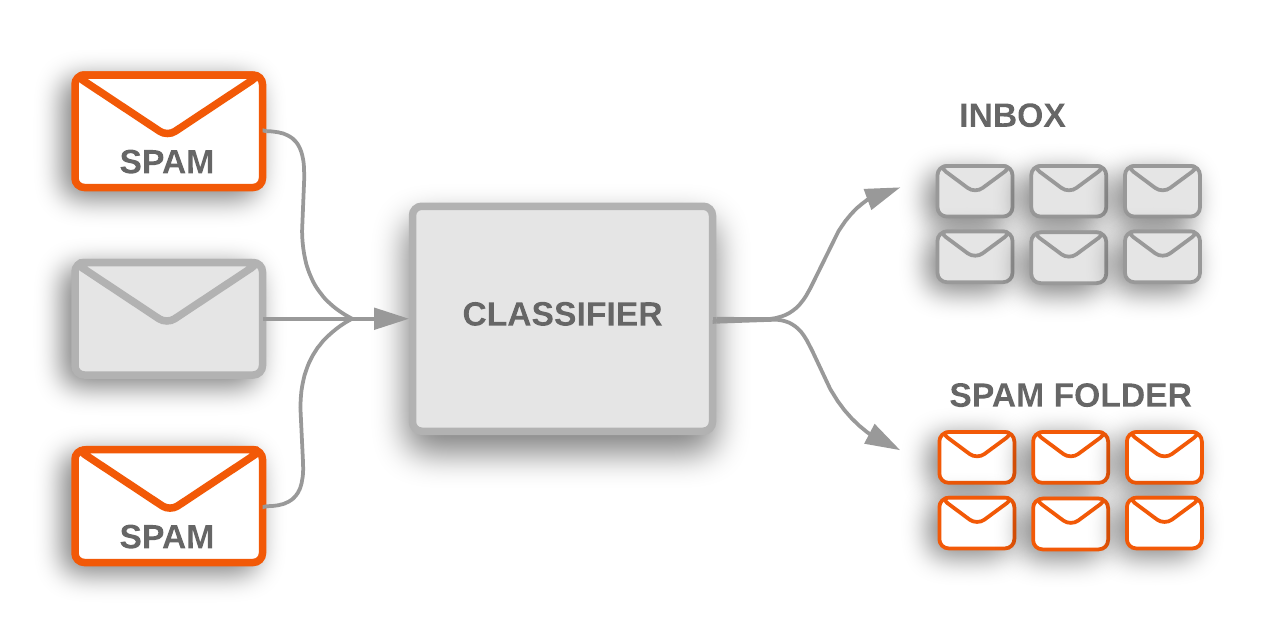
\includegraphics[width=\linewidth]{pic/Figure_30.png}
        \end{figure}
    \endminipage
\end{frame}

\begin{frame}{Real-World Example of Classification}
    \begin{itemize}
        \justifying
        \item \textbf{Pima Indians Diabetes Dataset:}
        \medskip
        \begin{itemize}\itemsep.8em
            \item \textbf{Problem}:
            Predict whether a patient has diabetes based on medical diagnostics.
            \item \textbf{Context}:
            Early detection of diabetes is critical for treatment and management.
        \end{itemize}
    \end{itemize}

    \begin{table}[]
        \resizebox{\textwidth}{!}{%
        \begin{tabular}{|c|c|c|c|c|c|c|c|c|c|}
\hline
\rowcolor[HTML]{C0C0C0} 
\cellcolor[HTML]{000000}                                                  & Number of times pregnant                          & Glucose                                           & Blood Pressure                                    & Skin Thickness                                    & Insulin                                           & Diabetes pedigree function                        & Age                                               & BMI                                               & Label                                             \\ \hline
\cellcolor[HTML]{C0C0C0}Patient 1                                         & 6                                                 & 148                                               & 72                                                & 35                                                & 0                                                 & 0.627                                             & 50                                                & 33.6                                              & \cellcolor[HTML]{FE0000}Positive                  \\ \hline
\cellcolor[HTML]{C0C0C0}Patient 2                                         & 1                                                 & 85                                                & 66                                                & 29                                                & 0                                                 & 0.351                                             & 31                                                & 26.6                                              & \cellcolor[HTML]{32CB00}Negative                  \\ \hline
\cellcolor[HTML]{C0C0C0}Patient 3                                         & 0                                                 & 137                                               & 40                                                & 35                                                & 168                                               & 2.288                                             & 33                                                & 43.1                                              & \cellcolor[HTML]{FE0000}Positive                  \\ \hline
\cellcolor[HTML]{C0C0C0}Patient 4                                         & 1                                                 & 89                                                & 66                                                & 23                                                & 94                                                & 0.167                                             & 21                                                & 28.1                                              & \cellcolor[HTML]{32CB00}Negative                  \\ \hline
\cellcolor[HTML]{C0C0C0}\begin{tabular}[c]{@{}c@{}}.\\ .\\ .\end{tabular} & \begin{tabular}[c]{@{}c@{}}.\\ .\\ .\end{tabular} & \begin{tabular}[c]{@{}c@{}}.\\ .\\ .\end{tabular} & \begin{tabular}[c]{@{}c@{}}.\\ .\\ .\end{tabular} & \begin{tabular}[c]{@{}c@{}}.\\ .\\ .\end{tabular} & \begin{tabular}[c]{@{}c@{}}.\\ .\\ .\end{tabular} & \begin{tabular}[c]{@{}c@{}}.\\ .\\ .\end{tabular} & \begin{tabular}[c]{@{}c@{}}.\\ .\\ .\end{tabular} & \begin{tabular}[c]{@{}c@{}}.\\ .\\ .\end{tabular} & \begin{tabular}[c]{@{}c@{}}.\\ .\\ .\end{tabular} \\ \hline
\end{tabular}
        %
        }
\end{table}



\end{frame}

\begin{frame}{Classification vs. Regression}
    \begin{table}[]
        \centering
        \begin{tabular}{|
        >{\columncolor[HTML]{C0C0C0}}c |c|c|}
        \hline
        \textbf{Aspect}        & \cellcolor[HTML]{C0C0C0}\textbf{Linear Regression}                                                & \cellcolor[HTML]{C0C0C0}\textbf{Linear Classification}                                           \\ \hline
        \textbf{Output Type}   & Continuous values (real numbers).                                                                 & \begin{tabular}[c]{@{}c@{}}Binary or Multi-class labels\\ (e.g., 0/1, A/B/C)\end{tabular}        \\ \hline
        \textbf{Use Cases}     & \begin{tabular}[c]{@{}c@{}}Predicting house prices,\\ stock market trends.\end{tabular}           & \begin{tabular}[c]{@{}c@{}}Email spam detection,\\ Credit Scoring, Churn Prediction\end{tabular} \\ \hline
        \end{tabular}
        \label{tab:my-table}
    \end{table}
\end{frame}


\section{Discriminant Functions}

\begin{frame}{Discriminant Functions in Machine Learning}
    \begin{itemize}
        \item \textbf{Definition}
        \medskip
        \begin{itemize}\itemsep1.5em
            \item \justifying A function that assigns a score to an input vector $x$, to classify it into different classes.
            \item \justifying It maps the input $\mathbf{x}$ to a real number $g(\mathbf{x})$, which represents the degree of confidence in assigning $\mathbf{x}$ to a particular class.
        \end{itemize}
    \end{itemize}
\end{frame}

\begin{frame}{Discriminant Functions in Machine Learning}
    \begin{itemize}
        \item \textbf{How it works}
        \medskip
        \begin{itemize}\itemsep1.5em
            \item \justifying \textbf{Binary Classification}: Two functions \textbf{$g_1(\mathbf{x})$} and \textbf{$g_2(\mathbf{x})$} for classes $C_1$ and $C_2$, respectively. The class is predicted by comparing these two functions:
            \[
                \hat{y} =
                \begin{cases} 
                    1 & \text{if } g_1(\mathbf{x}) > g_2(\mathbf{x}) \\
                    2 & \text{otherwise}
                \end{cases}
            \]

            \item \justifying \textbf{General Case}: For $k$-class problems, we compute \textbf{$g_i(\mathbf{x})$} for every class $i$, and assign \textbf{$x$} to class with highest score:
            $$
                \hat{y} = \arg \max_i g_i(\mathbf{x})
            $$
        \end{itemize}
    \end{itemize}
\end{frame}

\begin{frame}{Decision Boundary}
    \begin{itemize}
        \item \justifying \textbf{Definition}: A dividing hyperplane that separates different classes in a feature space, also known as "Decision Surface".
        \medskip
        \begin{figure}
            \centering
            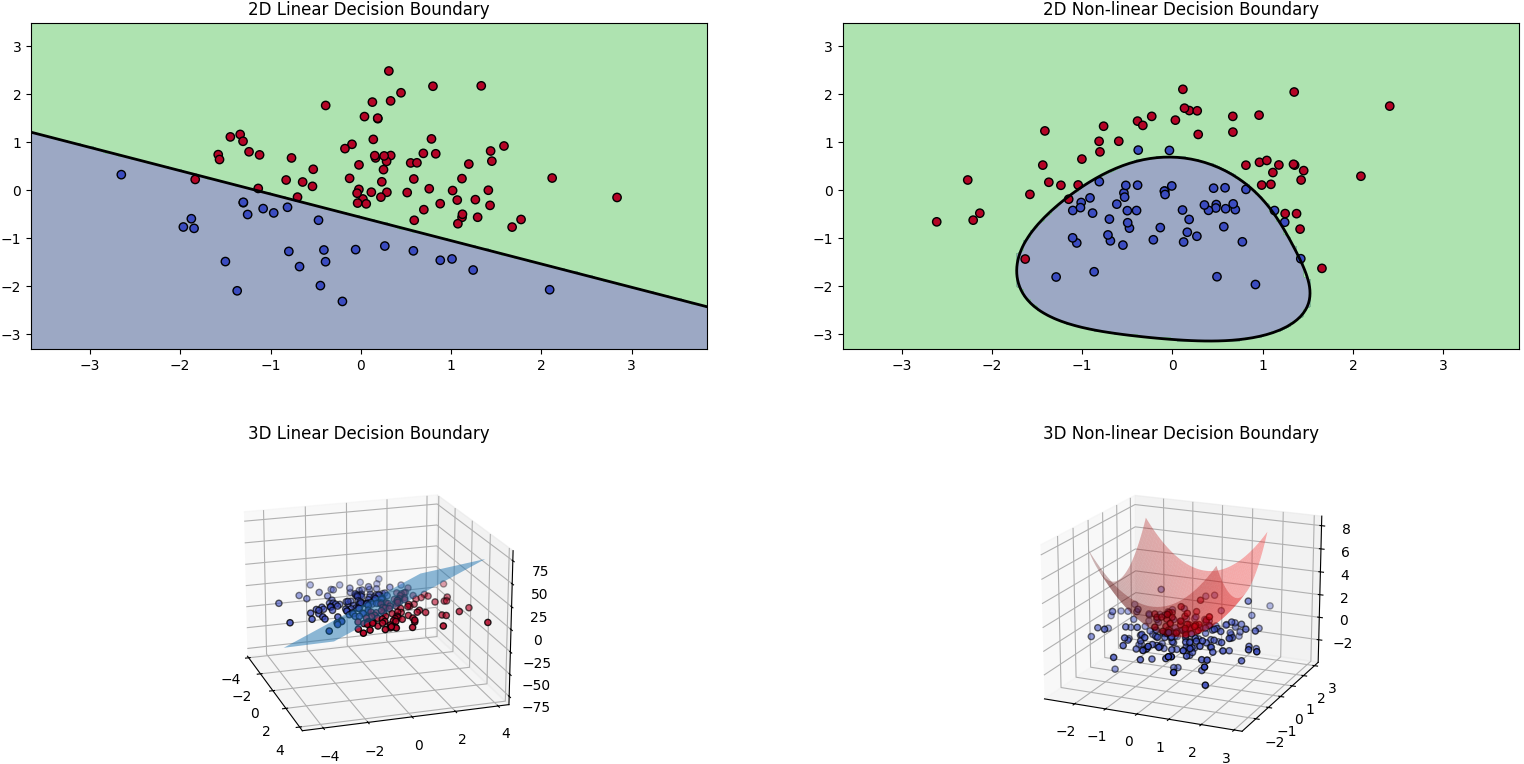
\includegraphics[width=.85\linewidth]{pic/Figure_24.png}
        \end{figure}
    \end{itemize}
\end{frame}

\begin{frame}{Discriminant Functions: Two-Category}
    \begin{itemize}\itemsep1.5em
        \item \justifying \textbf{Function}: For two-category problem, we can only find a function $g \, : \, \mathbb{R}^d \rightarrow \mathbb{R}$
        \begin{itemize}
            \item $g_1(\mathbf{x}) \, = \, g(\mathbf{x})$,
            \item $g_2(\mathbf{x}) \, = \, -g(\mathbf{x})$
        \end{itemize}
        \item \textbf{Decision Boundary}: $g(\mathbf{x}) \, = \, 0$
        \item \justifying At first, we start by explaining two-category classification for simplicity, and then extend the concept to multi-category classification for more complex problems.
    \end{itemize}
\end{frame}


\section{Linear Classifiers}

\begin{frame}{Linear Classifiers}
    \begin{itemize}\itemsep1.5em
        \item \justifying \textbf{Definition}: In case of linear classifiers, decision boundaries are linear in $d$ (\(\mathbf{x} \in \mathbb{R}^d\)), or linear in some given set of functions of $x$.
        \item \justifying \textbf{Linearly separable data}: Data points that can be exactly separated by a linear decision boundary.
        \item \textbf{Why are they popular?}
        \smallskip
        \begin{itemize}
            \item \justifying Simplicity, Efficiency, Effectiveness.
        \end{itemize}
    \end{itemize}
\end{frame}

\begin{frame}{Two Category Classification}
    \minipage{.5\textwidth}
    \begin{itemize}\itemsep1.5em
        \item \(g(\mathbf{x}) \, = \, \mathbf{w}^T\mathbf{x} + w_0 \, = \, w_d \cdot x_d + ... + w_1 \cdot x_1 + w_0\)
        \begin{itemize}
            \item \(\mathbf{x} = [x_1 \, \, ... \, \, x_d]\)
            \item \(\mathbf{w} = [w_1 \, \, ... \, \, w_d]\)
            \item \(w_0 \text{: bias}\)
        \end{itemize}
        \item \(
            \begin{cases} 
                C_1 & \text{if } \mathbf{w}^T\mathbf{x} + w_0 \geq 0 \\
                C_2 & \text{otherwise}
            \end{cases}
            \)
        \item \justifying \textbf{Decision Surface}: \(\mathbf{w}^T\mathbf{x} + w_0\)
    \end{itemize}
    \endminipage
    \hfill
    \minipage{.48\textwidth}
        \begin{figure}[bh]
            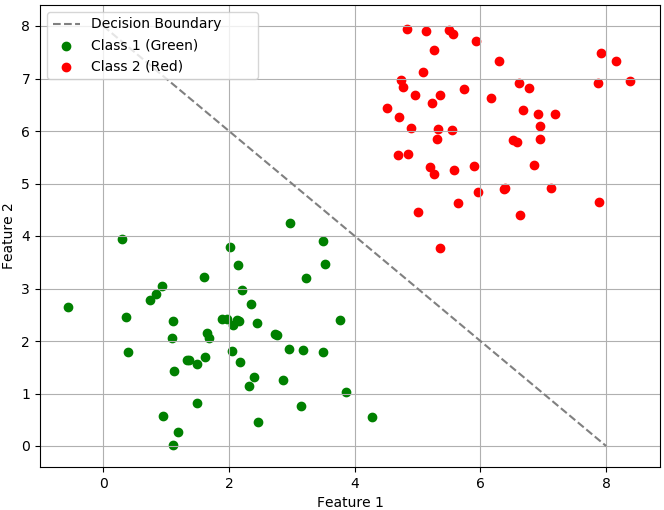
\includegraphics[width=\linewidth]{pic/Figure_1.png}
        \end{figure}
    \endminipage
\end{frame}


\begin{frame}{Two Category Classification Cont.}
    \begin{itemize}\itemsep1.5em
        \item Decision Boundary is a (\(d - 1\))-dimensional hyperplane \(H\) in the \(d\)-dimensional feature space. Some properties of \(H\) are:
        \medskip
        \begin{itemize}\itemsep0.7em
            \item Orientation of \(H\) is determined by the normal vector \([w_1 \, ... \, w_d]\) (\(\frac{w}{\Vert w \Vert}\)).
            \item \(w_0\) determines the location of the surface.
        \end{itemize}
    \end{itemize}
    \begin{figure}
        \centering
        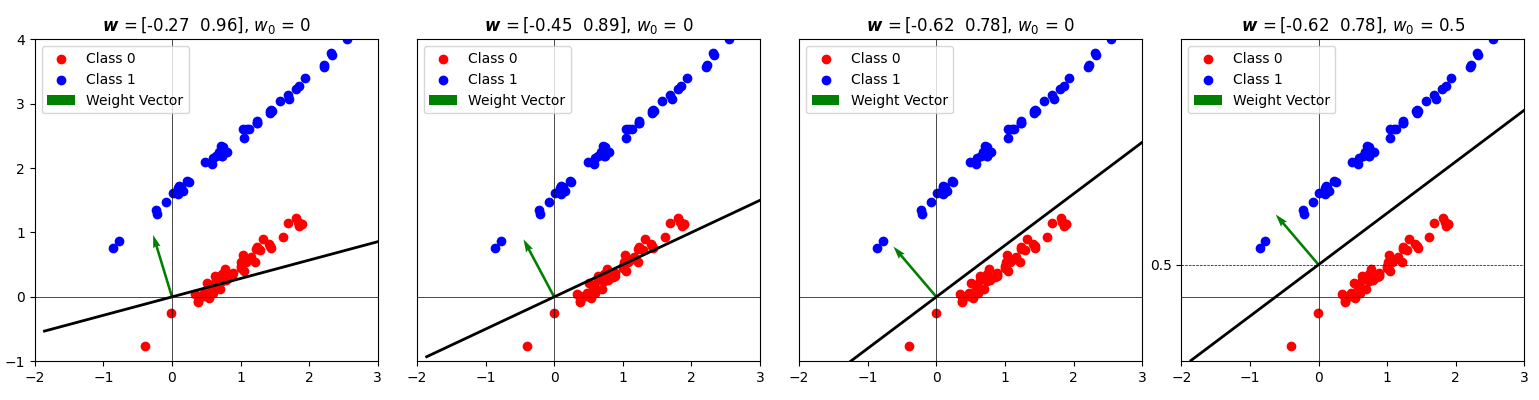
\includegraphics[width=\linewidth]{pic/Figure_25.png}
    \end{figure}
\end{frame}

\begin{frame}{Non-linear decision boundary}
    \minipage{.45\textwidth}
    \begin{itemize}
        \item \textbf{Non-linear Decision Boundaries}
        \begin{itemize}\itemsep1em
            \item \justifying \textbf{Feature Transformation}: Non-linearity is introduced by transforming features into a higher-dimensional space.
            \item \justifying \textbf{Linear in Transformed Space}: The decision boundary becomes linear in the new space, but non-linear in the original space.
        \end{itemize}
    \end{itemize}
    \endminipage
    \hfill
    \minipage{.5\textwidth}
        \begin{figure}[bh]
            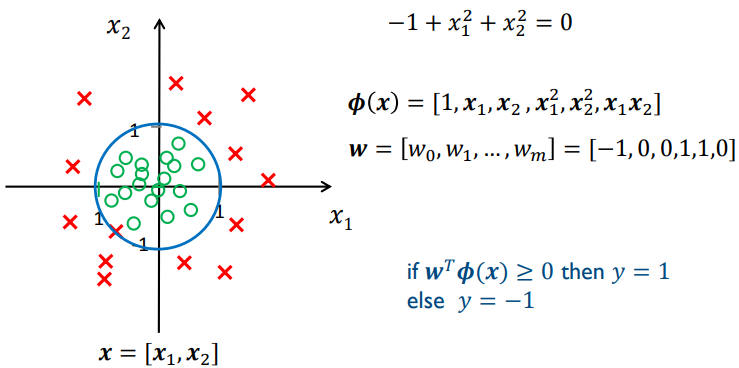
\includegraphics[width=\textwidth]{pic/Figure_10.png}
        \end{figure}
    \endminipage
\end{frame}

\section{Cost Functions}
\begin{frame}{Cost Functions}
    \begin{itemize}
        \item \textbf{Cost Functions in Linear Classifiers}
        \medskip
        \begin{itemize}\itemsep1em
            \item Purpose of cost functions is to measure the \textbf{difference} between \textbf{predicted} and \textbf{actual} class labels.
            \item Finding discriminant functions is framed as minimizing a cost function.
            \smallskip
            \begin{itemize}\itemsep0.8em
                \item Based on training set \(D \, = \, \{(\mathbf{x}^{(i)},\, y^{(i)})\}^N_{i=1},\) a cost function \(J(\mathbf{w})\) is defined.
                \item Problem converts to finding optimal \(\hat{g}(\mathbf{x}) \, = \, g(\mathbf{x; \hat{w}})\) where \[\mathbf{\hat{w}} \, = \, \arg \min_{\mathbf{w}}J(\mathbf{w})\]
            \end{itemize}
        \end{itemize}
    \end{itemize}
\end{frame}


\begin{frame}{Sum of Squared Error Cost Function}
    \begin{itemize}
        \item \textbf{Sum of Squared Error (SSE) Cost Function}\itemsep1em
        \medskip
        \begin{itemize}\itemsep0.8em
            \item \textbf{Formula}:
                \(
                J(\mathbf{w}) = \sum_{i=1}^{n} (y^{(i)} - \hat{y}^{(i)})^2 \, , \quad \hat{y}^{(i)} \, = \, \mathbf{w}^T\mathbf{x}^{(i)} \, + \, w_0
                \)
            \item \justifying SSE minimizes the magnitude of the error, which is ideal for \textbf{regression} but \textcolor{red}{irrelevant} for classification.
        \end{itemize}
    \end{itemize}
    \minipage{0.6\textwidth}
    \begin{itemize}
        \item \justifying If the model predicts close to the true class but not exactly 1 or -1, SSE still shows positive error, even for correct predictions.
    \end{itemize}
    \endminipage
    \minipage{.4\textwidth}
        \begin{figure}
            \centering
            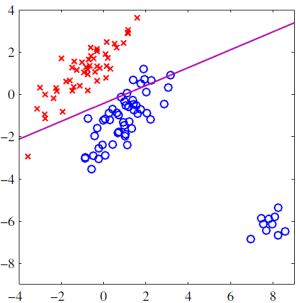
\includegraphics[width=.8\linewidth]{pic/Figure_11.png}
        \end{figure}
    \endminipage
\end{frame}


\begin{frame}{An Alternative for SSE Cost Function}
    \begin{itemize}
        \item \textbf{Number of Misclassifications}\itemsep1em
        \medskip
        \begin{itemize}\itemsep0.8em
            \item \textbf{Definition}:
            Measures how many samples are misclassified by the model.
            \item \textbf{Formula}:
                \[
                J(\mathbf{w}) = \sum_{i=1}^{n} (y^{(i)} - \text{sign(\(\hat{y}^{(i)})\)})^2 \, , \quad \hat{y}^{(i)} \, = \, \mathbf{w}^T\mathbf{x}^{(i)} \, + \, w_0
                \]
            \item \textbf{Limitations}: \\
            \minipage{0.5\linewidth}
            \begin{itemize}
                \item \justifying \textbf{Piecewise Constant}:
                The cost function is non-differentiable, so optimization techniques (like gradient descent) cannot be directly applied.
            \end{itemize}
            \endminipage
            \hspace{1cm}
            \minipage{0.28\textwidth}
            \begin{figure}[bh]
                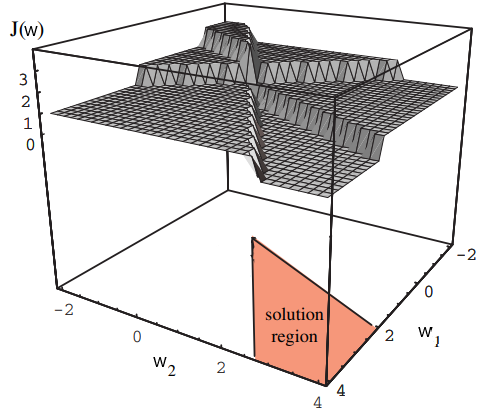
\includegraphics[width=\textwidth]{pic/Figure_12.png}
            \end{figure}
            \endminipage
        \end{itemize}
    \end{itemize}
\end{frame}


\begin{frame}{Perceptron Algorithm}
    \begin{itemize}
        \item \textbf{The Perceptron Algorithm}
        \medskip
        \begin{itemize}\itemsep1em
            \item \justifying \textbf{Purpose}:
            A simple algorithm for binary classification, separating two classes with a linear boundary.
        \end{itemize}
    \end{itemize}
    \begin{figure}
        \centering
        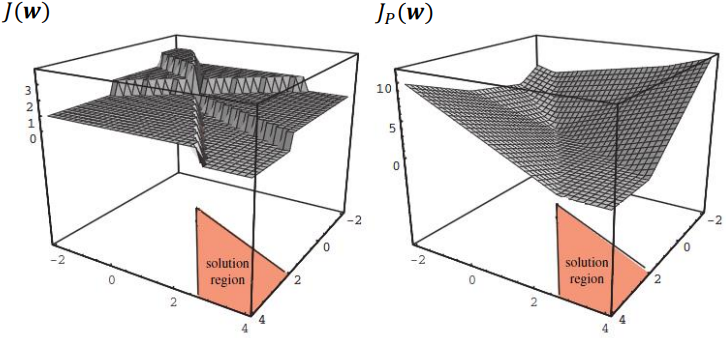
\includegraphics[width=0.7\linewidth]{pic/Figure_13.png}
    \end{figure}
\end{frame}


\begin{frame}{Perceptron Criterion}
    \begin{itemize}\itemsep1.2em
        \item \textbf{Cost Function}:
        The perceptron criterion focuses on misclassified points:
        \[
        J_p(\mathbf{w}) = - \sum_{i \in M} y^{(i)} \, \mathbf{w}^T \mathbf{x}^{(i)}
        \]
        where \( M \) is the set of misclassified points.
        \item \textbf{Goal}:
        Minimize the loss by correctly classifying all points.
    \end{itemize}
\end{frame}


\begin{frame}{Batch Perceptron}
    \begin{itemize}\itemsep1.5em
        \item \justifying \textbf{Batch Perceptron}:
        Updates the weight vector using all misclassified points in each iteration.
        \item \justifying \textbf{Gradient Descent}:
        Adjusting weights in the direction that reduces the loss:
        \[
        \mathbf{w} \leftarrow \mathbf{w} - \eta \nabla_\mathbf{w} \, J_p(\mathbf{w})
        \]
        \[
        \nabla_\mathbf{w} \, J_p(\mathbf{w}) \, = \, - \sum_{i \in M} y_i \mathbf{x}_i
        \]
        \begin{itemize}
            \item Batch Perceptron converges in finite number of steps for linearly separable data.
        \end{itemize}
    \end{itemize}
\end{frame}

\begin{frame}{Single-sample Perceptron}
    \begin{itemize}\itemsep1.5em
        \item \justifying \textbf{Single Sample Perceptron}: Updates the weight vector after each individual point.
        \item \textbf{Stochastic Gradient Descent (SGD) Update Rule:}
        \smallskip
        \begin{itemize}\itemsep1em
            \item Using only one misclassified sample at a time:
            \[
            \mathbf{w} \leftarrow \mathbf{w} + \eta y_i \mathbf{x}_i
            \]
            \item Lower computational cost per iteration, faster convergence.
            \item \justifying If training data are linearly separable, the single-sample perceptron is also guaranteed to find a solution in a finite number of steps.
        \end{itemize}
    \end{itemize}
\end{frame}

\begin{frame}{Example}
    \begin{itemize}
        \item Perceptron changes \(\mathbf{w}\) in a direction that corrects error.
    \end{itemize}
    \begin{figure}
        \centering
        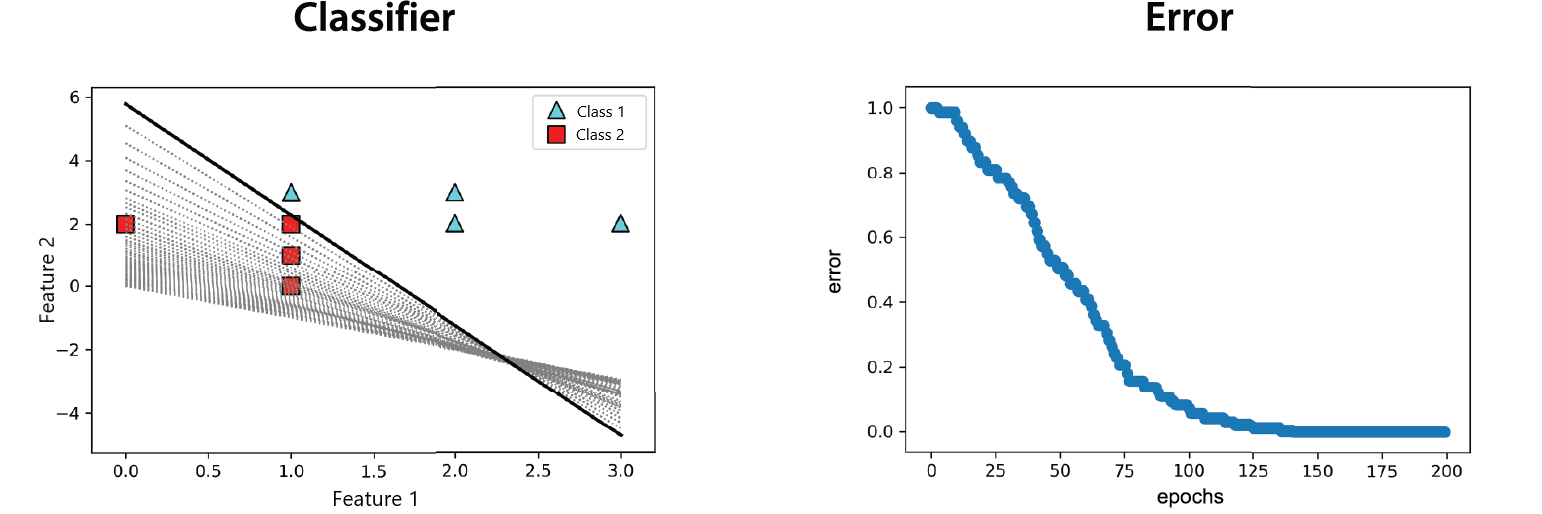
\includegraphics[width=\linewidth]{pic/Figure_14.png}
    \end{figure}
\end{frame}

\begin{frame}{Convergence of Perceptron}
    \begin{itemize}\itemsep1.5em
        \item \textbf{Non-Linearly Separable Data}:
        When no linear decision boundary can perfectly separate the classes, the Perceptron fails to converge.
        \medskip
        \begin{itemize}\itemsep1em
        \minipage{0.5\textwidth}
            \item If data is not linearly separable, there will always be some points that the model fails to classify.
            \item As a result, the algorithm keeps adjusting the weights to fix the misclassified points, causing it to never converge.
            \item For the data that are not linearly separable due to noise, \textbf{Pocket Algorithm} keeps in its pocket the best \(\mathbf{w}\) encountered up to now.
        \endminipage
        \minipage{0.4\textwidth}
        \hspace{1.5cm}
        \begin{figure}
            \centering
            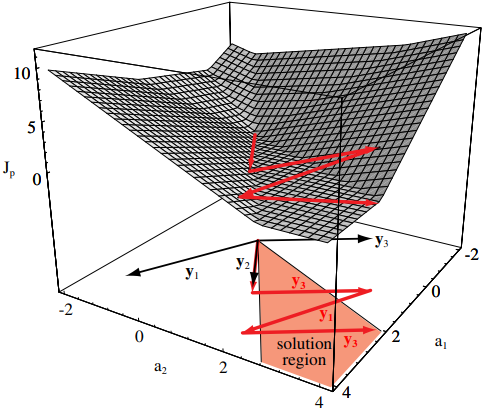
\includegraphics[width=.9\linewidth]{pic/Figure_15.png}
        \end{figure}
        \endminipage
        \end{itemize}
    \end{itemize}
\end{frame}

\begin{frame}{Pocket Algorithm}
    \begin{algorithm}[H]
    \caption{Pocket Algorithm}\label{alg:Pocket Algorithm}
    \begin{algorithmic}[1]
        \State \textbf{Initialize} $\mathbf{w}$
        \For{$t = 1$ to $T$}
            \State \(i \leftarrow t \text{ mod } N\)
            \If{\(\mathbf{x}^{(i)}\) is misclassified}
            \State \(\mathbf{w}^{new} \, = \, \mathbf{w} + \mathbf{x}^{(i)}y^{(i)}\)
            \If{\(E_{train}(\mathbf{w}^{new}) \, < \, E_{train}(\mathbf{w})\)}
            \State \(\mathbf{w} \, = \, \mathbf{w}^{new}\)
            \EndIf
            \EndIf
        \EndFor
    \end{algorithmic}
    \end{algorithm}
\end{frame}

\section{Perceptron}

\begin{frame}{But What Is Perceptron?}
    \minipage{.65\textwidth}
    \begin{itemize}
        \item \textbf{Perceptron Unit}:
        \medskip
        \begin{itemize}\itemsep1em
        \item \justifying \textbf{Basic Building Block}:
        A perceptron is the simplest type of artificial neuron used in machine learning.
        \item \justifying \textbf{Linear Classifier}:
        It maps input features to an output by applying a linear combination and a threshold.
        \item \justifying \textbf{Binary Decision}:
        Outputs 1 if the weighted sum of inputs exceeds the threshold, otherwise 0.
        \item \justifying \textbf{Components}:
        Inputs, weights, bias, and an activation function (often a step function).
        \end{itemize}
    \end{itemize}
    \endminipage
    \hfill
    \minipage{.3\textwidth}
    \begin{figure}
        \centering
        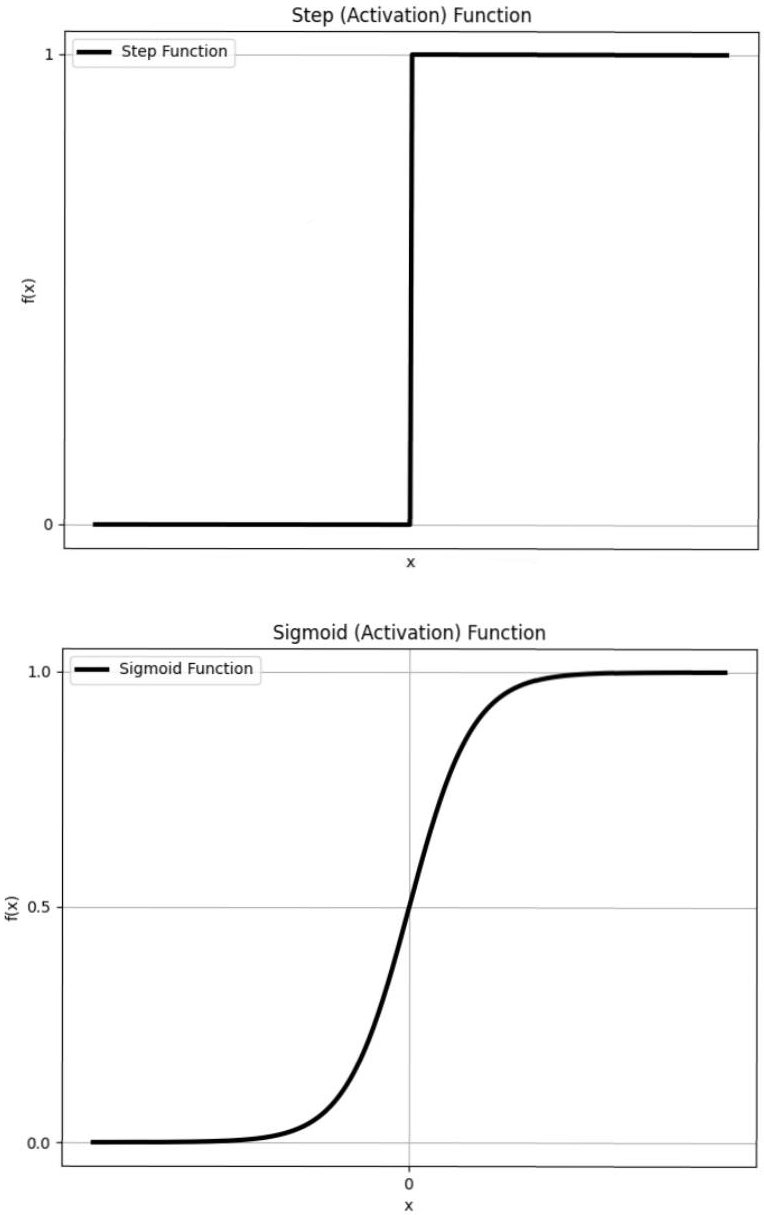
\includegraphics[width=.6\linewidth]{pic/Figure_17.png}
    \end{figure}
    \begin{figure}
        \centering
        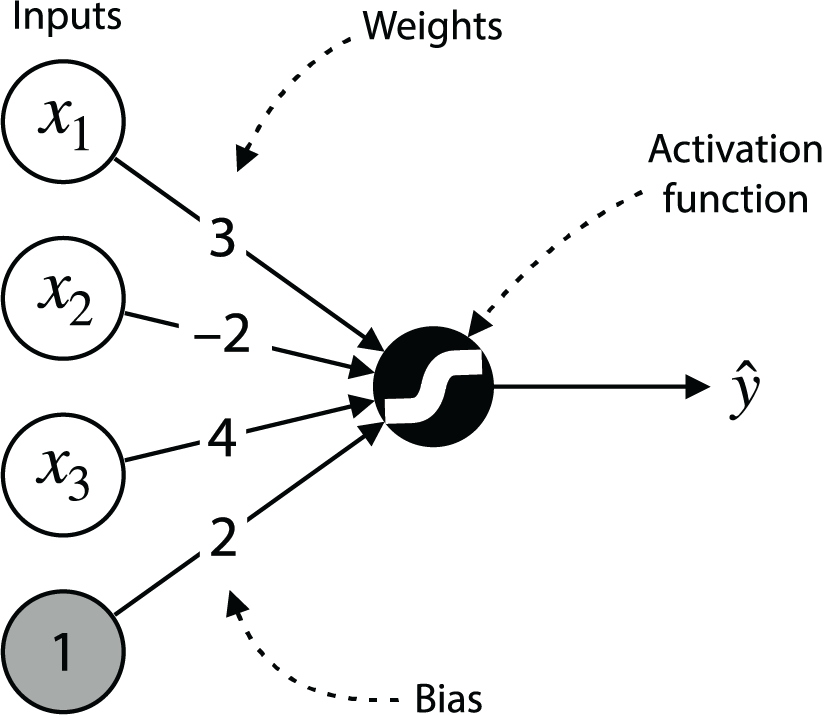
\includegraphics[width=0.6\linewidth]{pic/Figure_18.png}
    \end{figure}
    \endminipage
\end{frame}


\begin{frame}{Inspired by Biology}
    \begin{itemize}
        \item \textbf{Biological Motivation Behind Perceptron:}
        \medskip
        \begin{itemize}\itemsep1em
            \item \justifying \textbf{Inspired by Neurons}:
            Perceptron mimics the basic function of biological neurons in the brain.
            \begin{itemize}
                \item \justifying Input and Output, Activation Function.
            \end{itemize}
        \end{itemize}
    \end{itemize}
    \begin{figure}
        \centering
        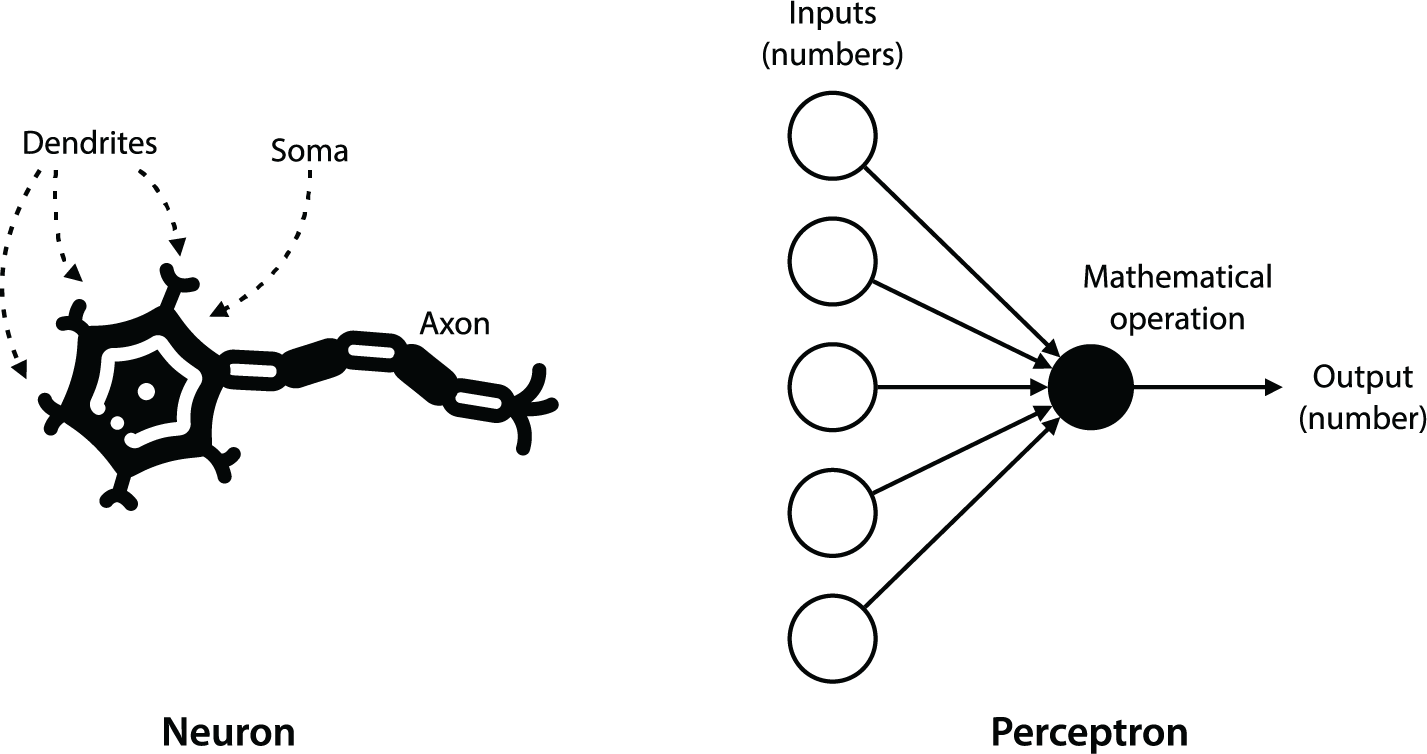
\includegraphics[width=0.55\linewidth]{pic/Figure_19.png}
    \end{figure}
\end{frame}

\begin{frame}{Single Neuron}
    \minipage{.66\textwidth}
    \begin{itemize}
        \item \textbf{Single Neuron as a Linear Decision Boundary}
        \medskip
        \begin{itemize}\itemsep1em
        \item \justifying \textbf{Mathematical Form}:
        The output of a single neuron is computed as:
        \[
        y = f(\mathbf{w}^T \mathbf{x} + w_0)
        \]
        where:
        \begin{itemize}
            \item \( \mathbf{x} \) is the input vector.
            \item \( \mathbf{w} \) is the weight vector.
            \item \( w_0 \) is the bias term.
            \item \( f \) is an activation function (e.g., step function).
        \end{itemize}
        
        \item \justifying \textbf{Linear Separation}: 
        If the activation function is a step function, the neuron defines a linear decision boundary:
        \(
        \mathbf{w}^T \mathbf{x} + w_0 = 0
        \)
        \item \textbf{Decision Rule}:
        Class 1 if \( \mathbf{w}^T \mathbf{x} + w_0 \geq 0 \), otherwise Class 2.
        \end{itemize}
    \end{itemize}
    \endminipage
    \hfill
    \minipage{.3\textwidth}
        \centering Class = \(f(\mathbf{w}^T \mathbf{x} + w_0)\)
        \begin{figure}
            \centering
            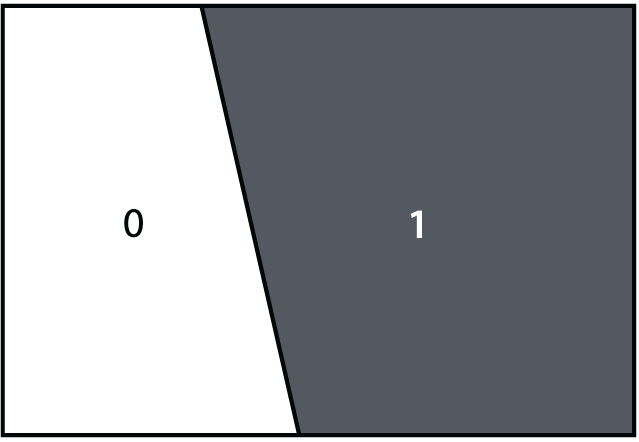
\includegraphics[width=\linewidth]{pic/Figure_20.png}
        \end{figure}
    \endminipage
\end{frame}

\begin{frame}{Limitations of a Single Perceptron}
    \begin{itemize}
        \item \textbf{What a Single Perceptron Can and Can't Do:}
        \medskip
        \begin{itemize}\itemsep1em
            \item \justifying \textbf{Performs Linear Separations:}
            A single perceptron can handle linearly separable problems such as:
            \begin{itemize}
                \item AND operation
                \item OR operation
            \end{itemize}
            \minipage{.6\textwidth}
            \item \justifying \textbf{Fails on Non-Linear Problems:}
            A single perceptron fails to solve non-linear problems like XOR, as the data points cannot be separated by a straight line.
            \endminipage
            \hfill
            \minipage{.3\textwidth}
            \begin{figure}
                \centering
                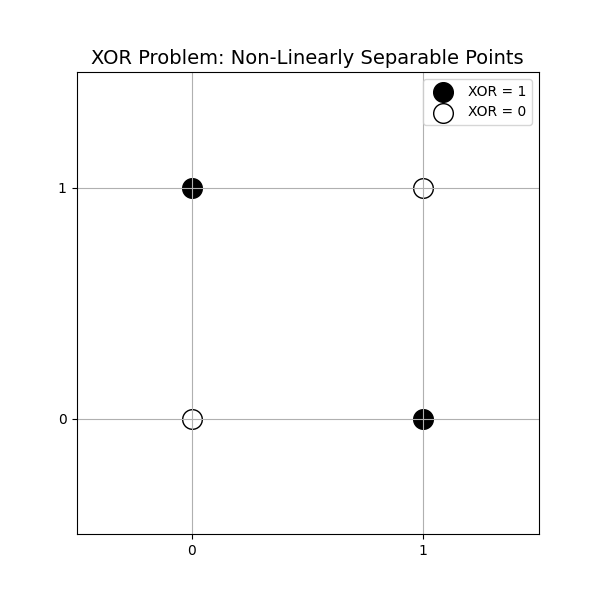
\includegraphics[width=\linewidth]{pic/Figure_23.png}
            \end{figure}
            \endminipage
        \end{itemize}
    \end{itemize}
\end{frame}



\begin{frame}{Towards Complex Decision Boundaries}
    \begin{itemize}
        \item \textbf{Multi-Layer Perceptron (MLP):}
        \medskip
        \begin{itemize}\itemsep1em
            \item \justifying \textbf{Adding Layers for More Complexity}:
            An MLP consists of multiple layers of neurons that allow us to model more complex functions than a single neuron.
            \begin{itemize}
                \item \justifying Each layer introduces new decision boundaries, making it possible to separate non-linear data.
            \end{itemize}
            \item \justifying \textbf{Two-Layer Example:}
            \begin{itemize}
                \item Input Layer $\rightarrow$ Hidden Layer $\rightarrow$ Output Layer
                \item Hidden layer introduces non-linear transformations that enable complex decision regions.
            \end{itemize}
        \end{itemize}
    \end{itemize}
    \begin{figure}
        \centering
        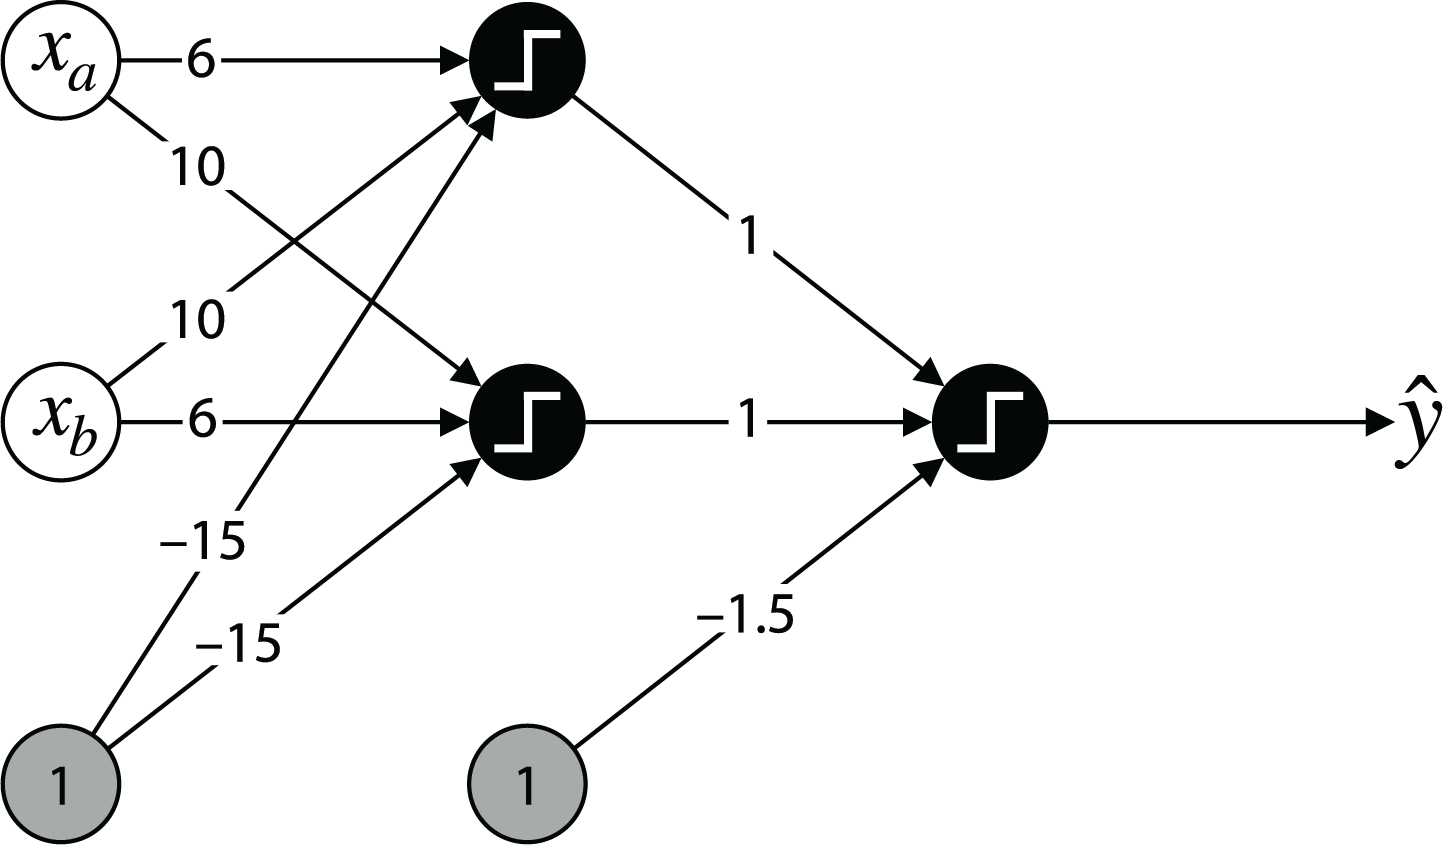
\includegraphics[width=0.38\linewidth]{pic/Figure_21.png}
    \end{figure}
\end{frame}


\begin{frame}{Refining the Decision Boundary}
    \begin{itemize}
        \item \justifying \textbf{New Neurons for Better Separation}:
        By adding more neurons to a layer, we can further refine the decision boundary to better separate complex data.
        \item \justifying Each additional neuron introduces new features that help the model make more accurate decisions.
    \end{itemize}
    \begin{figure}
        \centering
        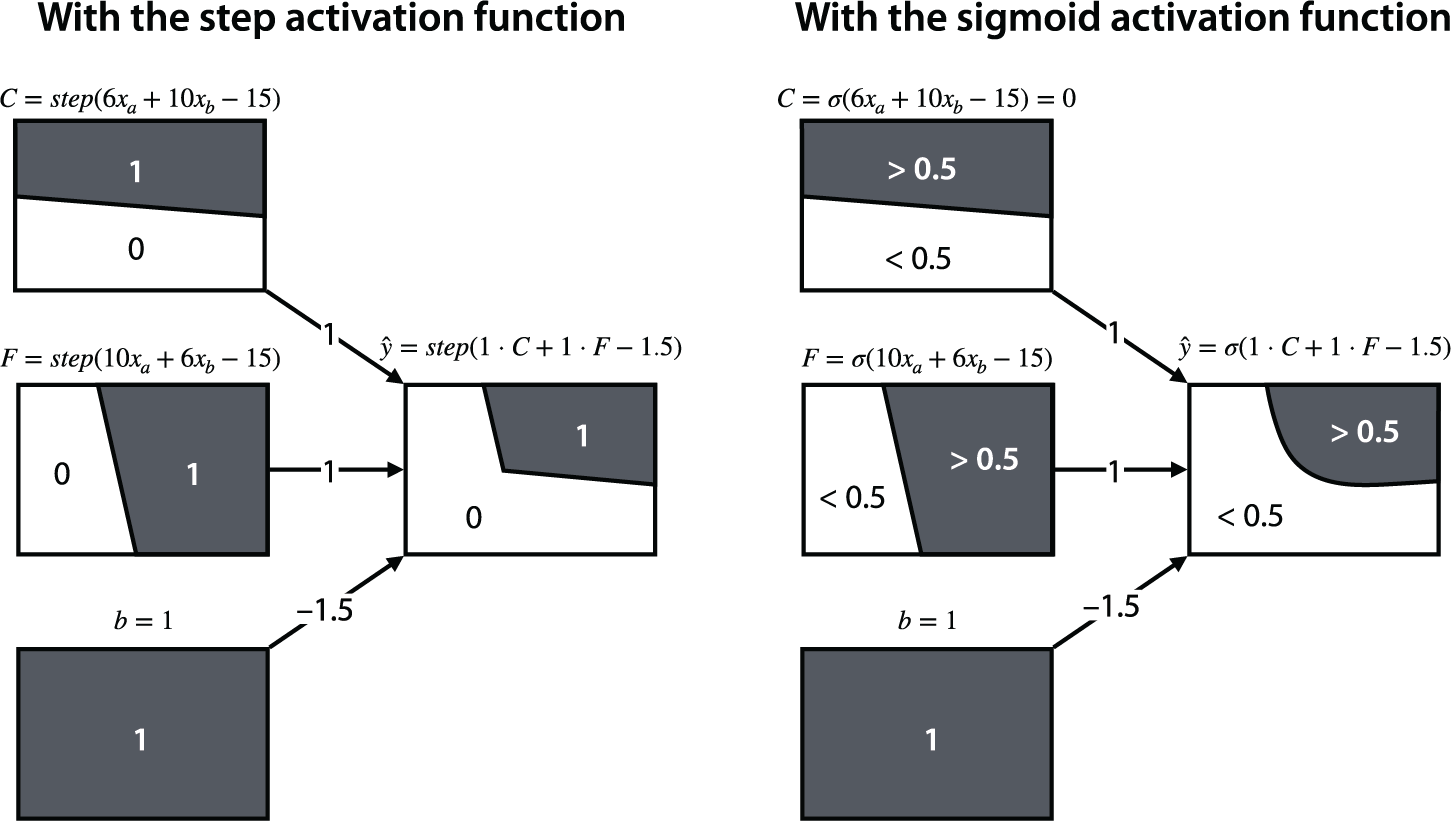
\includegraphics[width=0.53\linewidth]{pic/Figure_22.png}
    \end{figure}
\end{frame}



\section{Cross Validation}

\begin{frame}{Model Selection via Cross Validation}
    \begin{itemize}
        \item \textbf{Cross-Validation}
        \medskip
        \begin{itemize}\itemsep1em
            \item \justifying \textbf{Purpose}:
            Technique for evaluating how well a model generalizes to unseen data.
            \item \justifying \textbf{How It Works}:
            Split data into $k$ folds; train on $k-1$ folds and validate on the remaining fold.
            \item \justifying \textbf{Repeat Process}:
            Repeat $k$ times, rotating the test fold each time. Average of all scores is the final score of the model.
            \item \justifying Cross-validation
            reduces overfitting and provides a more reliable estimation of model performance.
        \end{itemize}
    \end{itemize}
\end{frame}


\begin{frame}{K-Fold Cross Validation}
    \begin{figure}
        \centering
        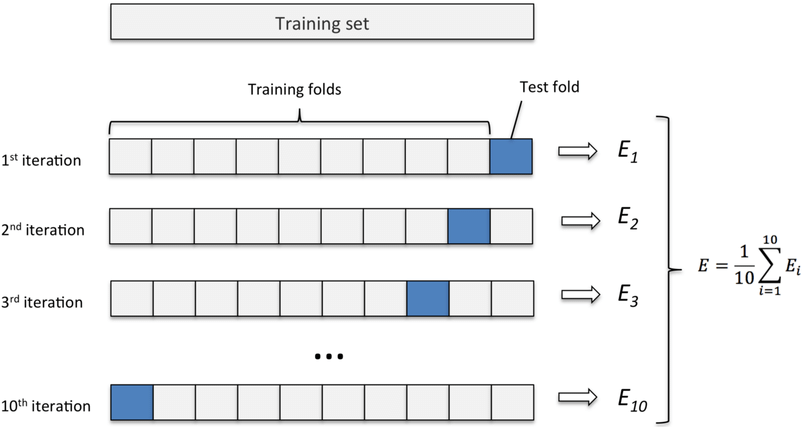
\includegraphics[width=.8\textwidth]{pic/Figure_28.png}
    \end{figure}
\end{frame}


\begin{frame}{Leave-One-Out Cross-Validation (LOOCV)}
    \begin{itemize}
        \item \textbf{Leave-One-Out Cross-Validation (LOOCV)}
            \medskip
            \begin{itemize}\itemsep1em
            \item \justifying \textbf{How It Works}:
            Uses a single data point as the validation set ($k$ = 1) and the rest as the training set. Repeat for all data points.
            \item \textbf{Properties:}
            \smallskip
            \begin{itemize}\itemsep.5em
                \item \textbf{No Data Wastage}:
                Every data point is used for both training and validation.
                \item \textbf{High Variance, Low Bias}.
                \item \justifying \textbf{Computationally Expensive}: 
                Requires training the model $N$ times for $N$ data points, making it slow for large datasets.
                \item \textbf{Best for small datasets}.
            \end{itemize}
        \end{itemize}
    \end{itemize}
\end{frame}

\begin{frame}{Cross-Validation for Choosing Regularization Term}
    \begin{figure}
        \centering
        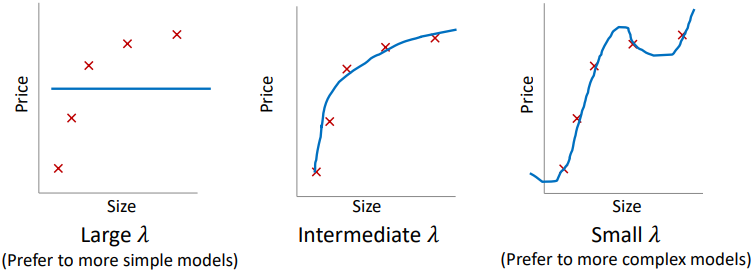
\includegraphics[width=0.8\linewidth]{pic/Figure_29.png}
    \end{figure}
\end{frame}

\begin{frame}{Cross-Validation for Choosing Model Complexity}
    \begin{figure}
        \centering
        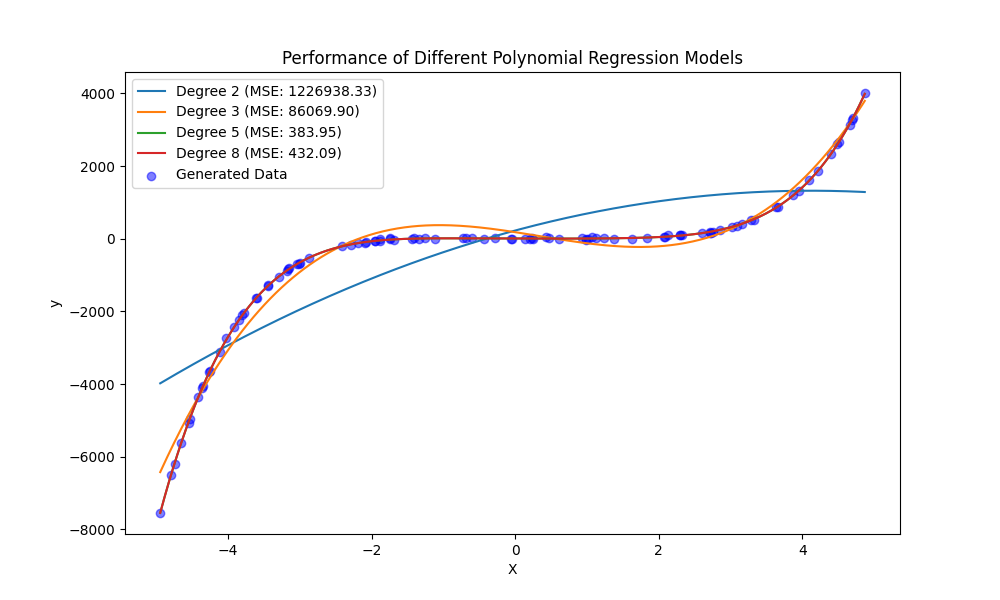
\includegraphics[width=0.8\linewidth]{pic/Figure_16.png}
    \end{figure}
\end{frame}

\section{Multi-Category Classification}

\begin{frame}{Multi-Category Classification}
    \begin{itemize}
        \item \textbf{Solutions to multi-category classification problem}:
        \medskip
        \begin{itemize}\itemsep1.5em
            \item Extend the learning algorithm to support multi-class.
            \medskip
            \begin{itemize}\itemsep1em
                \item First, a function \(g_i\) for every class \(C_i\) is found.
                \item Second, \(\mathbf{x}\) is assigned to \(C_i\) if \(g_i(\mathbf{x}) > g_j(\mathbf{x}) \quad \forall i \neq j\)
                \item[] \[\hat{y} \, = \, \argmax_{i=\text{1,...,c}} \, g_i(\mathbf{x})\]
            \end{itemize}
            \item Convert to a set of two-categorical problems.
            \medskip
            \begin{itemize}
                \item Methods like \textbf{One-vs-Rest} or \textbf{One-vs-One}, where each classifier distinguishes between either \textbf{one class and the rest}, or \textbf{between pairs of classes}.
            \end{itemize}
        \end{itemize}
    \end{itemize}
\end{frame}

\begin{frame}{Multi-Category Classification: Ambiguity}
    \begin{itemize}
        \item \justifying One-vs-One and One-vs-Rest conversion can lead to regions in which the classification is \textbf{undefined}.
    \end{itemize}
    \vfill
    \minipage{.45\textwidth}
    \begin{figure}[bh]
        \centering
        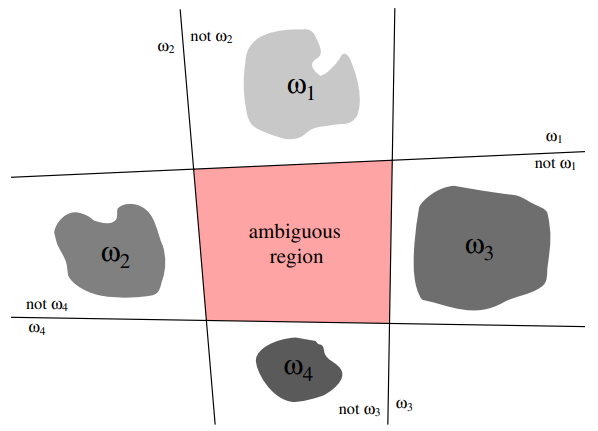
\includegraphics[width=\linewidth]{pic/Figure_6.png}
    \end{figure}
    \endminipage
    \minipage{.45\textwidth}
    \begin{figure}[bh]
        \centering
        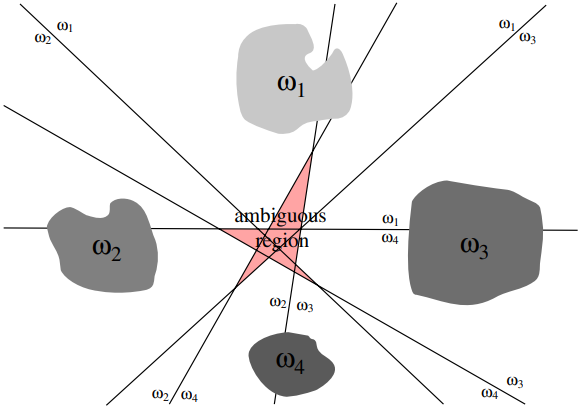
\includegraphics[width=\linewidth]{pic/Figure_7.png}
    \end{figure}
    \endminipage
\end{frame}


\begin{frame}{Multi-Category Classification: Linear Machines}
    \begin{itemize}\itemsep1.5em
        \item \justifying \textbf{Linear Machines}: Alternative to One-vs-Rest and One-vs-One methods; 
        Each class is represented by its own discriminant function.
        \item \justifying \textbf{Decision Rule:} 
        \[\hat{y} \, = \, \argmax_{i=\text{1,...,c}} \, g_i(\mathbf{x})\]
        The predicted class is the one with the highest discriminant function value.
        \item \textbf{Decision Boundary}:
        \(g_i(\mathbf{x}) \, = \, g_j(\mathbf{x})\)
        \[(\mathbf{w}_i - \mathbf{w}_j)^T\mathbf{x} + (w_{0i} - w_{0j}) = 0\]
    \end{itemize}
\end{frame}


\begin{frame}{Linear Machines Cont.}
    \begin{center}
        \minipage{.5\textwidth}
            \begin{figure}
                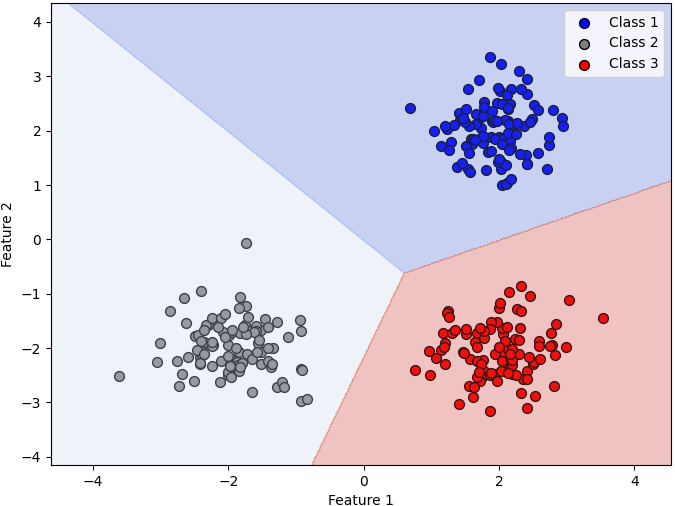
\includegraphics[width=\textwidth]{pic/Figure_9.png}
            \end{figure}
        \endminipage
    \end{center}
    \hspace{4cm}
    \begin{itemize}\itemsep1.5em
        \item \justifying The decision regions of this discriminant are \textbf{convex} and \textbf{singly connected}. Any point on the line between two points within the same region can be expressed as 
\(
\mathbf{x} = \lambda \mathbf{x}_A + (1 - \lambda) \mathbf{x}_B
\)
where \( \mathbf{x}_A, \mathbf{x}_B \in C_k \).

    \end{itemize}
\end{frame}

\begin{frame}{Multi-Class Perceptron Algorithm}
    \begin{itemize}
        \item \textbf{Weight Vectors}:
        \medskip
        \begin{itemize}\itemsep.8em
            \item Maintain a weight matrix \( W \in \mathbb{R}^{m \times K} \), where \( m \) is the number of features and \( K \) is the number of classes.
        \item Each column \( w_k \) of the matrix corresponds to the weight vector for class \( k \).
        \end{itemize}
    \end{itemize} \\
    \[
    \hat{y} \, = \, \argmax_{i=1,...,c} \, \mathbf{w}_i^T \mathbf{x}
    \]
    \[
    J_p(\mathbf{W}) \, = \, - \sum_{i \in M}(\mathbf{w}_{y^{(i)}} - \mathbf{w}_{\hat{y}^{(i)}})^T\mathbf{x}^{(i)}
    \]
    where \( M \) is the set of misclassified points.
\end{frame}


\begin{frame}{Multi-Class Perceptron Algorithm}

    \begin{algorithm}[H]
    \caption{Multi-class perceptron}\label{alg:Multi-class perceptron}
    \begin{algorithmic}[1]
        \State \textbf{Initialize} $\mathbf{W} \, = \, [\mathbf{w}_1 \, , \, ... \, , \, \mathbf{w}_c], \, k \leftarrow 0$
        \While{A pattern is misclassified}
            \State \(k \leftarrow k \, + \, 1 \text{ mod } N\)
            \If{\(\mathbf{x}^{(i)}\) is misclassified}
            \State \(\mathbf{w}_{\hat{y}^{(i)}} \, = \, \mathbf{w}_{\hat{y}^{(i)}} - \mathbf{x}^{(i)}\)
            \State \(\mathbf{w}_{y^{(i)}} \, = \, \mathbf{w}_{y^{(i)}} + \mathbf{x}^{(i)}\)
            \EndIf
        \EndWhile
    \end{algorithmic}
    \end{algorithm}
    
\end{frame}


\section{References}

\begin{frame}[allowframebreaks]
    \bibliography{ref}
    \bibliographystyle{ieeetr}
    \nocite{*} % used here because no citation happens in slides
    % if there are too many try use:
    % \tiny\bibliographystyle{alpha}
\end{frame}

\end{document}